\documentclass[a4paper,12pt,twoside,final,spanish]{article}
%titlepage: pone el título en una página aparte
%twocolumn
\usepackage{babel} %Para el lenguaje [spanish]
\usepackage[utf8]{inputenc} %Para reconocer todos los símbolos
\usepackage[T1]{fontenc}
\usepackage{textcomp}
\usepackage{amsmath}
\usepackage[makeroom]{cancel} %Para tachar expresiones matemáticas
\usepackage{xcolor}
\newcommand\Ccancel[2][black]{\renewcommand\CancelColor{\color{#1}}\cancel{#2}}
\usepackage{amsfonts}
\usepackage{amssymb}
\usepackage[margin=2cm]{geometry} %Márgenes
\usepackage[T1]{fontenc}
\usepackage{graphicx}
\usepackage{hyperref}
\usepackage{enumerate} %Para cambiar los items de numeración
\usepackage{soul} % para tachar texto
\pagestyle{headings}
% Para encerrar expresiones con círculos
\usepackage{mathtools}% superior to amsmath
\usepackage{tikz}
\makeatletter
\newcommand\mathcircled[1]{%
  \mathpalette\@mathcircled{#1}%
}
\newcommand\@mathcircled[2]{%
  \tikz[baseline=(math.base)] \node[draw,circle,inner sep=1pt] (math) {$\m@th#1#2$};%
}
\makeatother
%---
\usepackage{fancyhdr} %Para usar encabezados y pies personalizados
	\pagestyle{fancy}
	\fancyhf{}
	\fancyhead[LE,RO]{Mecánica del Continuo}
	\fancyhead[RE,LO]{Tensiones}
	\fancyfoot[LE,RO]{\thepage}
	\fancyfoot[RE,LO]{Darién Julián Ramírez}	
	\renewcommand{\footrulewidth}{1pt}
%---

\title{\Huge Mecánica del Continuo\\
Trabajo Práctico Nº3\\
Tensiones}
\author{Darién Julián Ramírez}
\date{\vspace{-5ex}}

\begin{document}

\maketitle %Crea la página de título

\section*{Ejercicio 1}

Tome una tiza y rómpala por:
\begin{enumerate}[a.]
\item Flexión.
\item Torsión.
\end{enumerate}

La forma en que rompe la tiza será diferente en cada caso. ¿Por qué? ¿Se puede predecir el modo de falla? ¿La superficie de rotura?

\dotfill

\begin{quote}

La forma en que rompe la tiza es diferente en cada caso porque la fuerza se encuentra aplicada de manera distinta.

Tanto el modo de falla como la superficie de rotura son predecibles:

\begin{enumerate}[a.]
\item Flexión:

\begin{center}
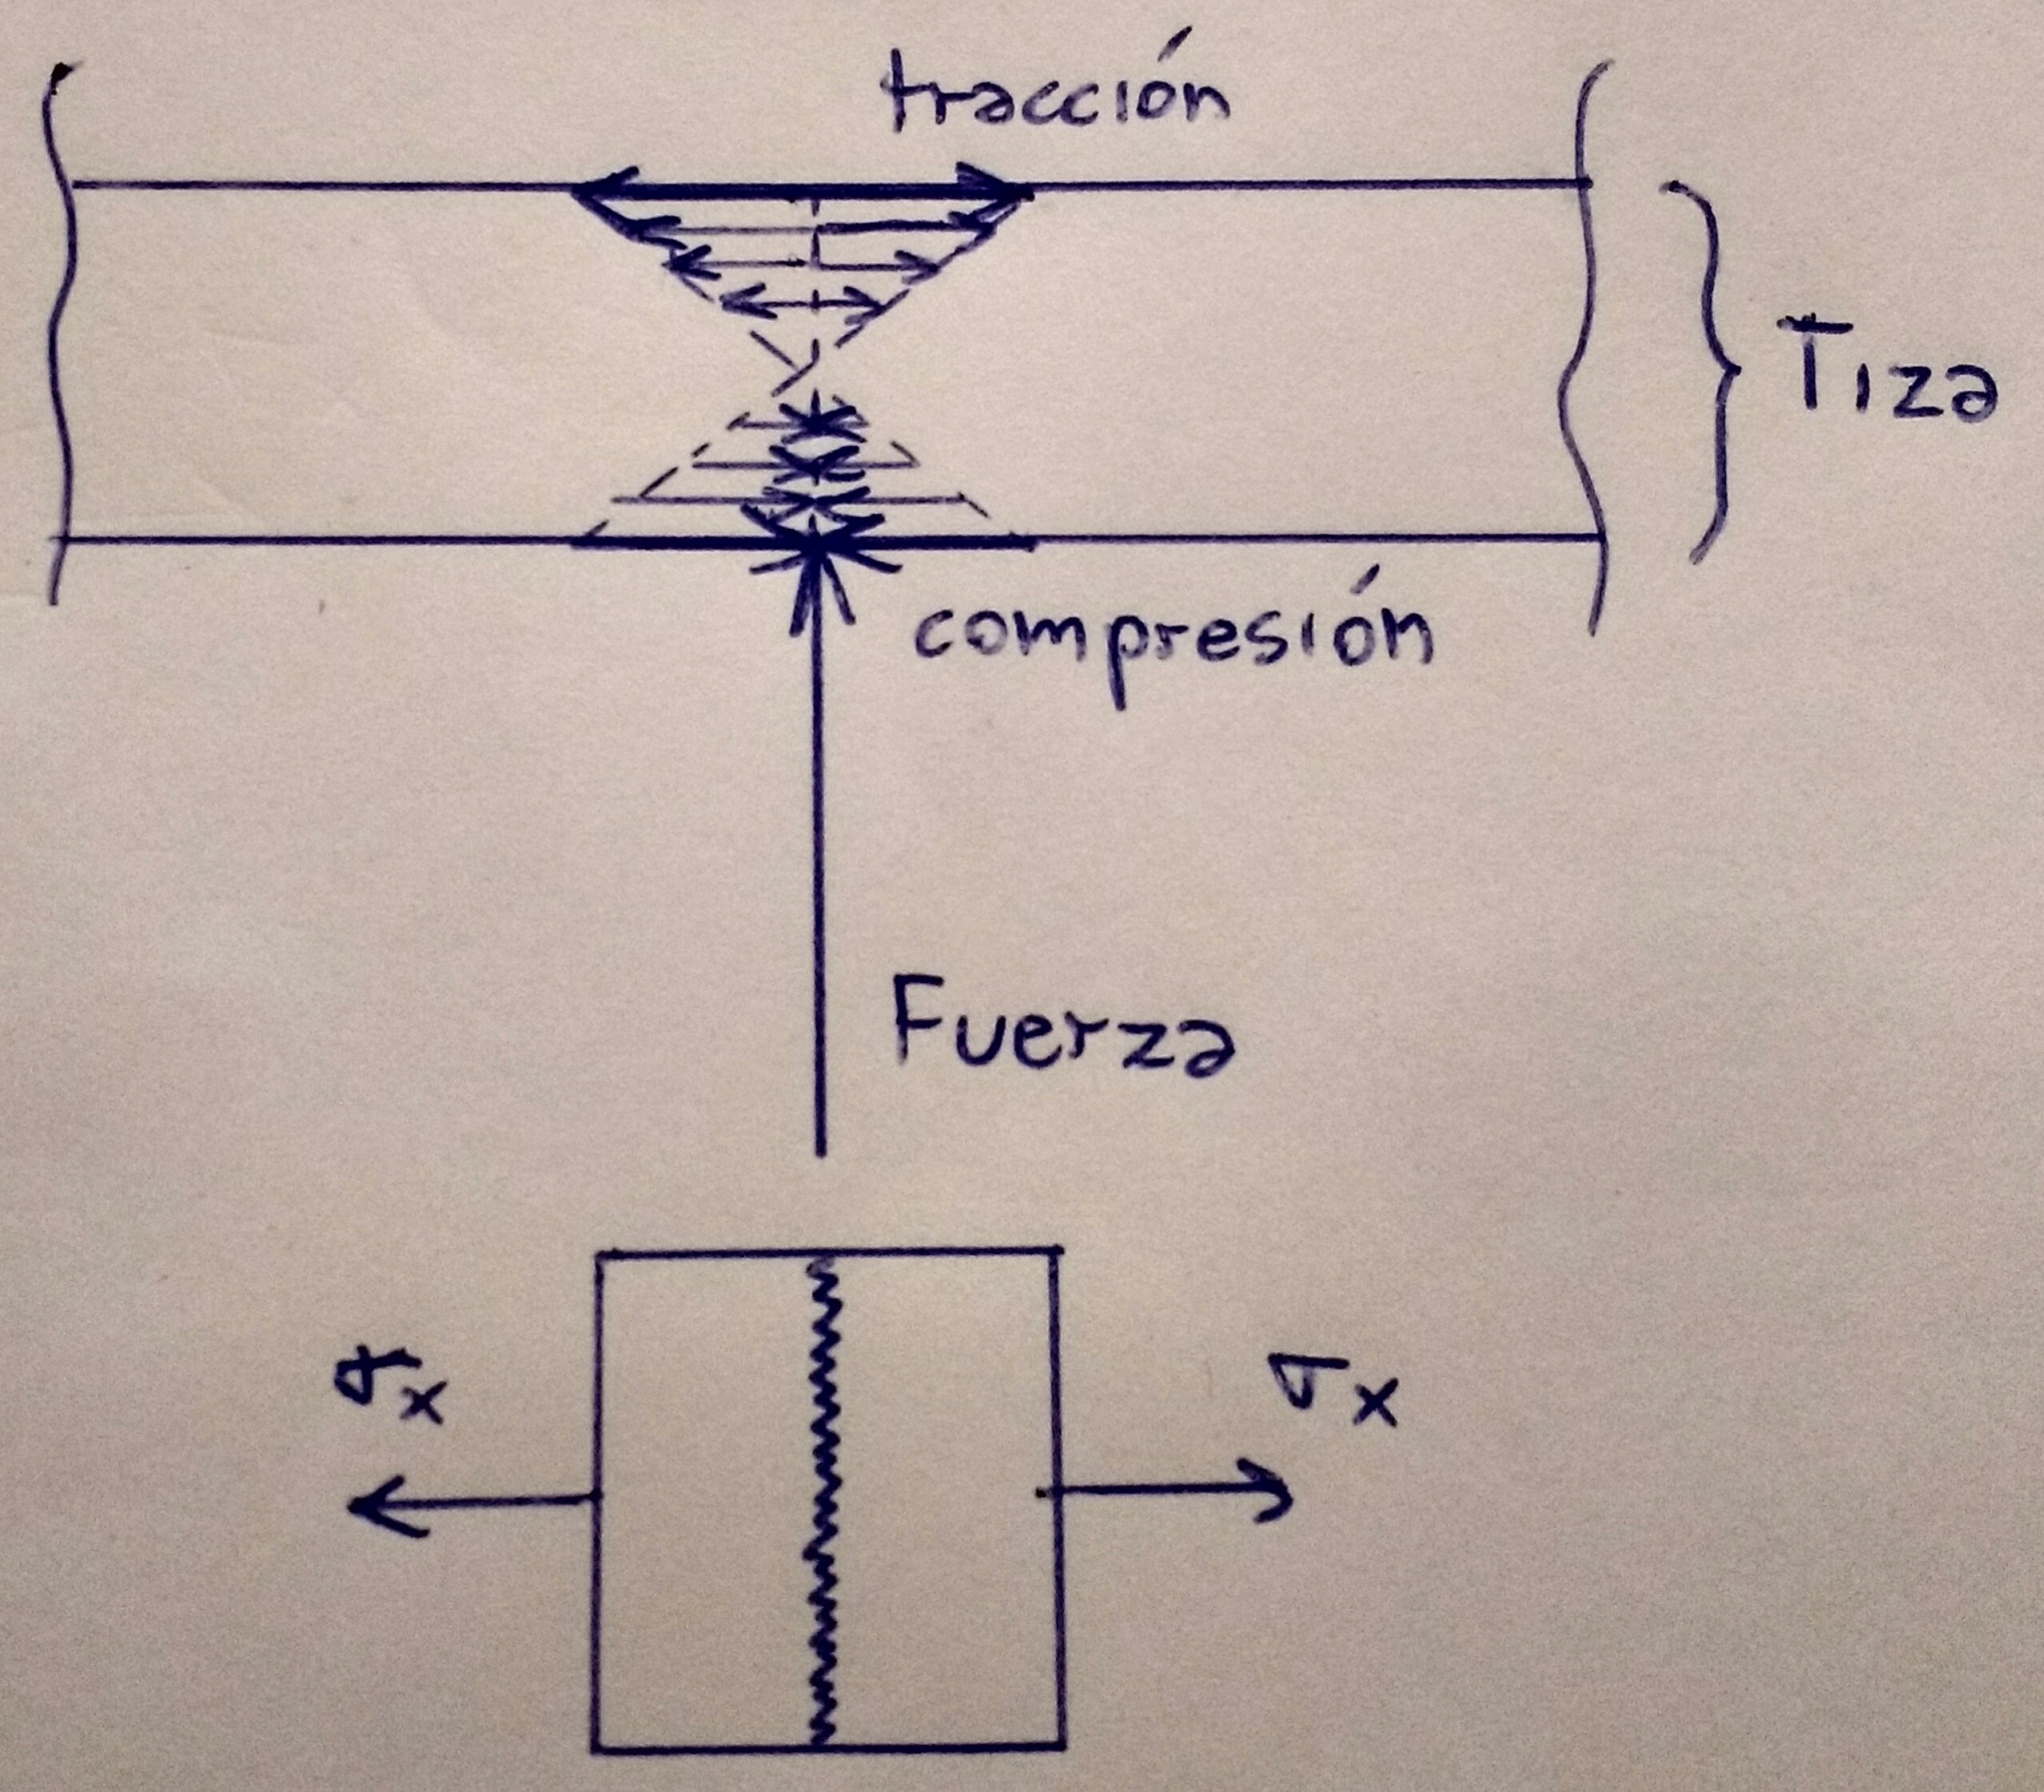
\includegraphics[width=0.5\linewidth,keepaspectratio]{4.jpg}
\end{center}

Hipótesis Euler-Bernoulli:

\[
\left(\begin{matrix}
\sigma_{x} & 0 & 0\\
0 & 0 & 0\\
0 & 0 & 0\\
\end{matrix}\right)
\]

\item Torsión:

\begin{center}
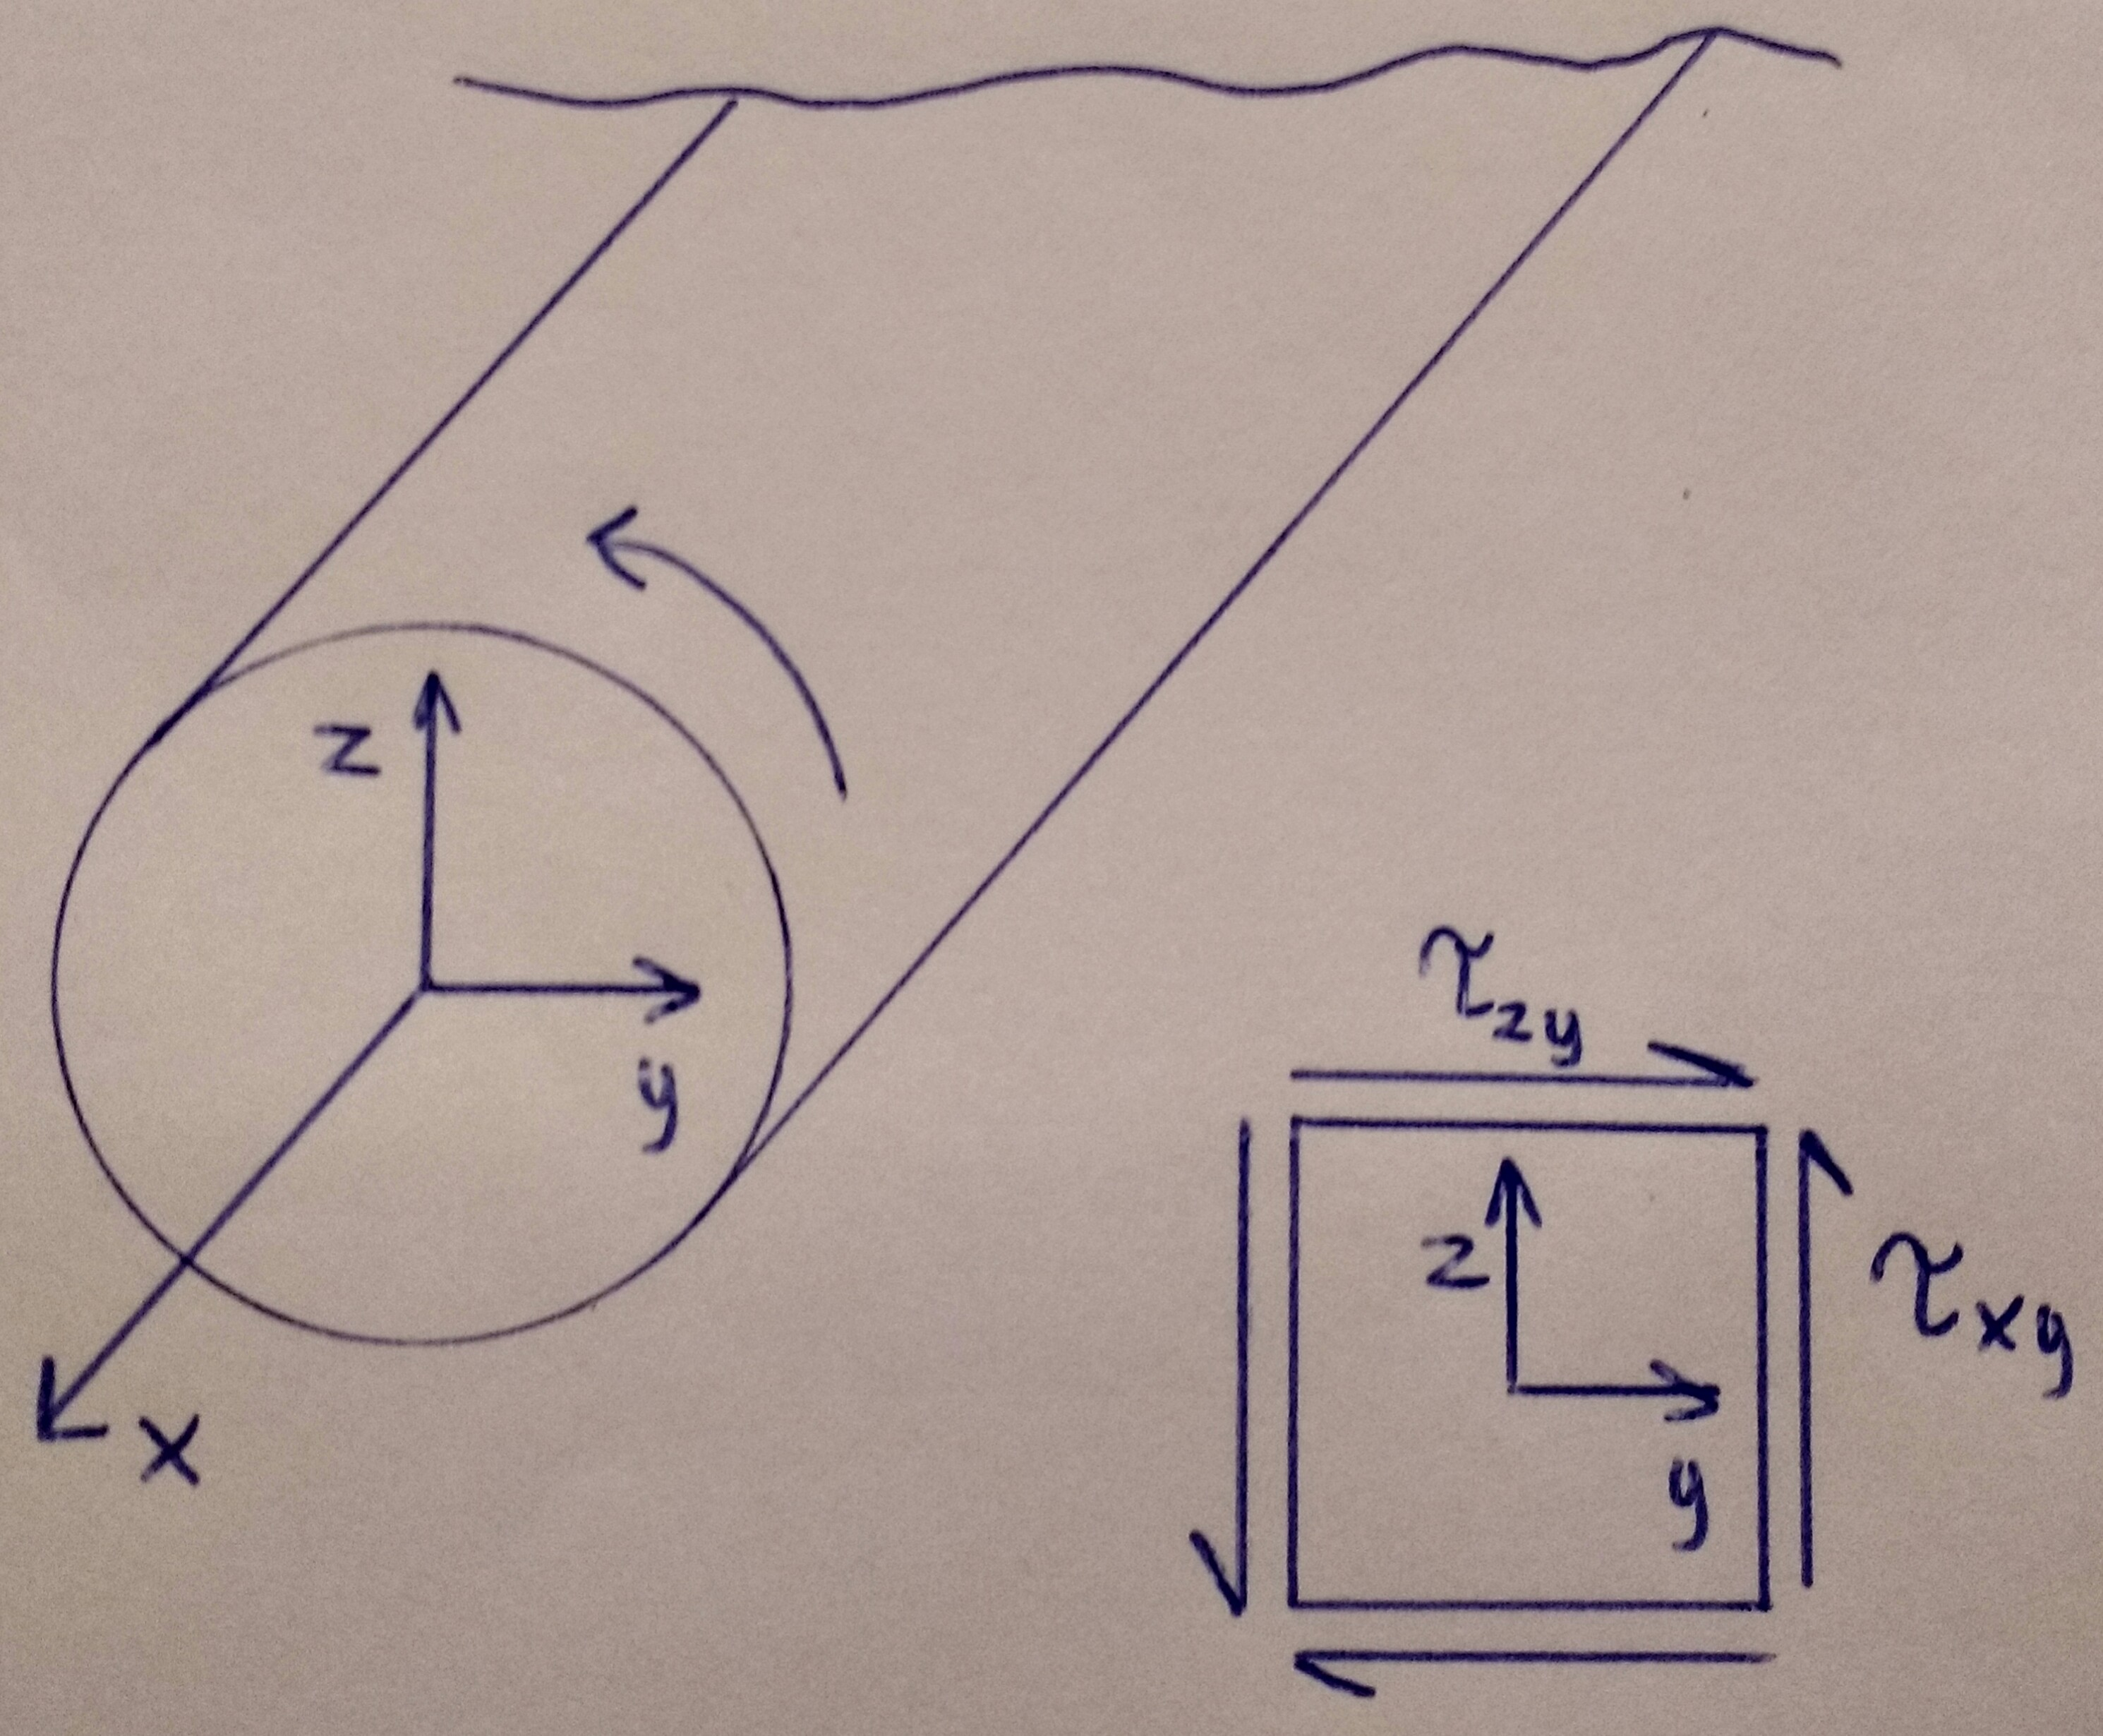
\includegraphics[width=0.5\linewidth,keepaspectratio]{5.jpg}
\end{center}

Hipótesis de Coulomb:

\[
\left(\begin{matrix}
0 & 0 & 0\\
0 & 0 & \tau_{yz}\\
0 & \tau_{zy} & 0\\
\end{matrix}\right)
\]
\end{enumerate}
\end{quote}

\section*{Ejercicio 2}

La figura muestra agua en un reservorio. En un punto $P$, consideremos las superficies 
$A-A$, $B-B$, etc. Dibuje los vectores de tensión que actúan sobre estas superficies. 
Considere todas las posibles superficies que pasen por $P$. ¿Cuál es el lugar geométrico de todos los vectores de tensión? 

\begin{center}
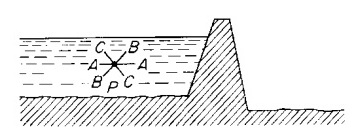
\includegraphics[width=0.5\linewidth,keepaspectratio]{1.jpg}
\end{center}

\textit{Rta: una esfera}

\dotfill

\begin{quote}

Densidad del agua: $\rho_{a}$\\
Gravedad: $g$\\
Profundidad: $h$

El punto es comprimido con igual magnitud desde todas las direcciones:

\[
\sigma_{ij}=
\left(\begin{matrix}
-\rho_{a}gh & 0 & 0\\
0 & -\rho_{a}gh & 0\\
0 & 0 & -\rho_{a}gh\\
\end{matrix}\right)
=(-\rho_{a}gh)\delta_{ij};\quad\textit{Presión hidroestática}
\]

$\tau_{ij}'=\beta_{ie}\beta_{jm}\tau_{em}=\beta_{ie}\beta_{jm}(-\rho_{a}gh)\delta_{em}=\beta_{ie}\beta_{je}(-\rho_{a}gh)=(-\rho_{a}gh)\delta_{ij}$

El lugar geométrico de todos los vectores de tensión resulta ser una esfera.

\end{quote}

\section*{Ejercicio 3}

El agua de un reservorio desborda por un vertedero. Considere un punto próximo a la 
pared superior del vertedero, digamos a 10 cm sobre el mismo. Considere nuevamente 
todas las superficies que pasan por este punto y describa los vectores de tensión que 
actúan sobre estas superficies. ¿Es nuevamente el lugar geométrico de estos vectores 
una esfera?\\

Considere ahora una sucesión de puntos que se acerca de la superficie de superior del 
vertedero, digamos a distancias 1 cm, 0,1 cm, 0,01 cm, 0,001 cm,  etc. ¿Esperaría 
usted que el lugar geométrico de los vectores de tensión cambie cuando la distancia se 
hace muy pequeña? Preste atención a la viscosidad del agua.

\begin{center}
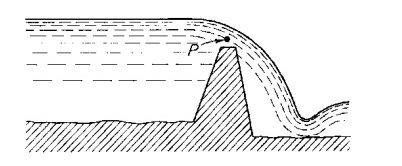
\includegraphics[width=0.5\linewidth,keepaspectratio]{2.jpg}
\end{center}

\dotfill \\

En agua en movimiento, el tensor de tensiones depende de la velocidad y la viscosidad. Aparece la presión dinámica. El lugar geométrico del vector de tensión no es una esfera.

\section*{Ejercicio 4}

Las componentes del tensor de tensiones en un cierto punto de un cuerpo, pueden ser 
presentadas como una matriz: 

\[
\left(\begin{matrix}
0 & 1 & 2\\
1 & 2 & 0\\
2 & 0 & 1\\
\end{matrix}\right)
\]

¿Cuál es el vector de tensión que actúa en el lado externo (el lado opuesto al origen) 
del plano siguiente, que pasa por el punto en cuestión? 

\[x+3y+z=1\]

¿Cuáles son las componentes normales y tangenciales del vector de tensión en este 
plano? 

\dotfill

\begin{quote}


Primero es necesario determinar el versor normal $\nu$. Teniendo la ecuación del plano, el vector normal al plano se define como:

\[
ax+by+cz+d=0\implies \mathbf{n}=
\left(\begin{matrix}
a \\
b \\
c \\
\end{matrix}\right)
=
\left(\begin{matrix}
1 \\
3 \\
1 \\
\end{matrix}\right)
\]

El vector $\mathbf{n}$ es normal al plano pero no es unitario, entonces:

\[
\nu=\frac{\mathbf{n}}{\|\mathbf{n}\|}=\frac{(a,b,c)^{T}}{\sqrt{a^2+b^2+c^2}}
=\frac{(1,3,1)^{T}}{\sqrt{1^2+3^2+1^2}}=\frac{(1,3,1)^{T}}{\sqrt{11}}
=\left(\frac{1}{\sqrt{11}},\frac{3}{\sqrt{11}},\frac{1}{\sqrt{11}}\right)^{T}
\]

Ahora es posible calcular el vector de tensión:

\[
\stackrel \nu T_{i}=\sigma_{ij}\nu_{j}=\frac{1}{\sqrt{11}}\cdot
\left(\begin{matrix}
0 & 1 & 2\\
1 & 2 & 0\\
2 & 0 & 1\\
\end{matrix}\right)\cdot
\left(\begin{matrix}
1 \\
3 \\
1 \\
\end{matrix}\right)=\frac{1}{\sqrt{11}}\cdot
\left(\begin{matrix}
5 \\
7 \\
3 \\
\end{matrix}\right)
\]

Se calcularán las componentes normal y tangencial de vector de tensión:

\[
\stackrel \nu T=T^{(n)}+T^{(c)}\implies=T^{(c)}=\stackrel \nu T-T^{(n)}
\]

\[
T^{(n)}=(\stackrel \nu T\cdot\nu)\nu=\left(
\frac{1}{\sqrt{11}}
\left(\begin{matrix}
5 \\
7 \\
3 \\
\end{matrix}\right)\cdot
\frac{1}{\sqrt{11}}
\left(\begin{matrix}
1 \\
3 \\
1 \\
\end{matrix}\right)\right)
\frac{1}{\sqrt{11}}
\left(\begin{matrix}
1 \\
3 \\
1 \\
\end{matrix}\right)=
\frac{29}{11}\cdot
\frac{1}{\sqrt{11}}
\left(\begin{matrix}
1 \\
3 \\
1 \\
\end{matrix}\right)
\]

\[
T^{(c)}=\stackrel \nu T-T^{(n)}=
\frac{1}{\sqrt{11}}
\left(\begin{matrix}
5 \\
7 \\
3 \\
\end{matrix}\right)-
\frac{29}{11}\cdot
\frac{1}{\sqrt{11}}
\left(\begin{matrix}
1 \\
3 \\
1 \\
\end{matrix}\right)=\frac{1}{\sqrt{11}}\cdot
\left(\frac{26}{11},-\frac{10}{11},\frac{4}{11}\right)^{T}
\]

\end{quote}

\section*{Ejercicio 5}

Un cuerpo sometido a la siguiente distribución de tensiones, ¿se encuentra en equilibrio en ausencia de cargas de cuerpo?

\[
\sigma_{x}=3x^{2}+4xy-8y^{2};\quad\tau_{xy}=-\frac{1}{2}x^{2}-6xy-2y^{2}
\]

\[
\sigma_{y}=2x^{2}+xy+3y^{2};\quad\sigma_{z}=\tau_{xz}=\tau_{yz}=0
\]

\dotfill

\begin{quote}

Se tiene un estado plano de tensiones pues no hay fuerzas actuando en la dirección $z$.\\

Planteando las ecuaciones de equilibrio:\\
$\tau_{ji,j}+X_{i}=0\hfill\textit{Como no hay cargas de cuerpo, $X_{i}=0$}.\\
\tau_{ji,j}=0$

Para i=1: $\tau_{11,1}+\tau_{21,2}+\tau_{31,3}=\tau_{11,1}+\tau_{21,2}
=6x+4y-6x-4y=0$

Para i=2: $\tau_{12,1}+\tau_{22,2}+\tau_{32,3}=\tau_{12,1}+\tau_{22,2}
=-x-6y+x+6y=0$

Para i=3: $\tau_{13,1}+\tau_{23,2}+\tau_{33,3}=0$

El cuerpo se encuentra en equilibrio en ausencia de cargas de cuerpo.

\end{quote}

\section*{Ejercicio 6}

Si el estado de tensiones en un punto $(x_{0},y_{0},z_{0})$ es:

\[\sigma_{ij}=
\left(\begin{matrix}
100 & 0 & 0\\
0 & 50 & 0\\
0 & 0 & -100\\
\end{matrix}\right)
\]

hallar el vector de tensiones y la magnitud de la tensión normal y la tensión de corte 
actuando en el plano $x-x_{0}+y-y_{0}+z-z_{0}=0$.

\dotfill

\[
\nu=\frac{\mathbf{n}}{\|\mathbf{n}\|}=\frac{(a,b,c)^{T}}{\sqrt{a^2+b^2+c^2}}
=\frac{(1,1,1)^{T}}{\sqrt{1^2+1^2+1^2}}=\frac{(1,1,1)^{T}}{\sqrt{3}}
=\left(\frac{1}{\sqrt{3}},\frac{1}{\sqrt{3}},\frac{1}{\sqrt{3}}\right)^{T}
\]

\[
\stackrel \nu T_{i}=\sigma_{ij}\nu_{j}=\frac{1}{\sqrt{3}}\cdot
\left(\begin{matrix}
100 & 0 & 0\\
0 & 50 & 0\\
0 & 0 & -100\\
\end{matrix}\right)\cdot
\left(\begin{matrix}
1 \\
1 \\
1 \\
\end{matrix}\right)=\frac{1}{\sqrt{3}}\cdot
\left(\begin{matrix}
100 \\
50 \\
-100 \\
\end{matrix}\right)
\]

\[
T^{(n)}=(\stackrel \nu T\cdot\nu)\nu=\left(
\frac{1}{\sqrt{3}}
\left(\begin{matrix}
100 \\
50 \\
-100 \\
\end{matrix}\right)\cdot
\frac{1}{\sqrt{3}}
\left(\begin{matrix}
1 \\
1 \\
1 \\
\end{matrix}\right)\right)
\frac{1}{\sqrt{3}}
\left(\begin{matrix}
1 \\
1 \\
1 \\
\end{matrix}\right)=
\frac{50}{3}\cdot
\frac{1}{\sqrt{3}}
\left(\begin{matrix}
1 \\
1 \\
1 \\
\end{matrix}\right)
\]

\[
\|T^{(n)}\|=\frac{50}{3}
\]

\[
T^{(c)}=\stackrel \nu T-T^{(n)}=
\frac{1}{\sqrt{3}}
\left(\begin{matrix}
100 \\
50 \\
-100 \\
\end{matrix}\right)-
\frac{50}{3}\cdot
\frac{1}{\sqrt{3}}
\left(\begin{matrix}
1 \\
1 \\
1 \\
\end{matrix}\right)=\frac{1}{\sqrt{3}}\cdot
\left(\frac{250}{3},\frac{100}{3},-\frac{350}{3}\right)^{T}
\]

\[
\|T^{(c)}\|=84.984
\]

\section*{Ejercicio 7}

El conjunto de ocho planos con direcciones normales $(\pm 1,\pm 1,\pm 1)$, en donde se elige uno de los signos $+$ o – en cada caso, por ejemplo $(+1,+1,-1)$ corresponde  al plano $x+y-z=0$, es llamado conjunto de planos octaédricos. Sea un estado de tensión en un punto dado por $\tau_{ij}$, con $\tau_{ij}=0$ cuando $i\neq j$. Determinar el vector de tensiones y la tensión de corte actuando en cada uno de los planos octaédricos. 

\dotfill

\[
\nu=\left(\pm\frac{1}{\sqrt{3}},\pm\frac{1}{\sqrt{3}},\pm\frac{1}{\sqrt{3}}\right)^{T}\implies \stackrel \nu T_{i}=\tau_{ij}\nu_{j}=\frac{1}{\sqrt{3}}
\left(\begin{matrix}
\pm\tau_{11} \\
\pm\tau_{22} \\
\pm\tau_{33} \\
\end{matrix}\right)
\]

\[
T^{(n)}=(\stackrel \nu T\cdot\nu)\nu
=\frac{1}{3\sqrt{3}}(\pm\tau_{11}^{2}\pm\tau_{22}^{2}\pm\tau_{33}^{2})
\left(\begin{matrix}
\pm 1 \\
\pm 1 \\
\pm 1 \\
\end{matrix}\right)
\]

\[
T^{(c)}=\stackrel \nu T-T^{(n)}=\frac{1}{\sqrt{3}}
\left[\left(\begin{matrix}
\pm \tau_{11} \\
\pm \tau_{22} \\
\pm \tau_{33} \\
\end{matrix}\right)-\frac{1}{3}(\pm\tau_{11}^2\pm\tau_{22}^2\pm\tau_{33}^2)
\left(\begin{matrix}
\pm 1 \\
\pm 1 \\
\pm 1 \\
\end{matrix}\right)
\right]
\]

\section*{Ejercicio 8}

\textit{Flujo Couette.} El espacio entre dos cilindros concéntricos está lleno con un fluido. El cilindro interno está fijo, en tanto el cilindro externo rota con una velocidad angular $\omega\left[\frac{rad}{seg}\right]$. Si el torque medido en el cilindro interno  es  $T$, ¿cuánto vale el torque medido en el cilindro exterior? ¿Porqué? 

\begin{center}
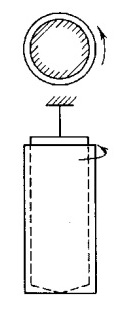
\includegraphics[width=0.15\linewidth,keepaspectratio]{3.jpg}
\end{center}

\dotfill

\begin{quote}
$T$: torque $[N.m]$\\

Traslación: $\sum F=\frac{d}{dt}(mv)=m\frac{dv}{dt}=ma$\\

Rotación: $\sum M=\frac{d}{dt}(I\omega)=I\frac{d\omega}{dt}=ma$; $\hfill I$: momento de inercia.\\

Si $\omega=cte\implies\frac{d\omega}{dt}=0\implies\sum M=0$\\

En el fluido: $M_{ext}-M_{int}=0\implies M_{ext}=M_{int}=T$
\end{quote}

\section*{Ejercicio 9}

Enrolle una hoja de papel formando un cilindro circular de radio del orden de 3 a 5 cm. Este tubo puede soportar una compresión axial apreciable.

Coloque el tubo sobre la mesa y comprímalo axialmente con la palma de la mano. El 
cilindro fallará en un modo llamado pandeo. Describa la forma del pandeo. ¿Qué tan 
grande es la carga de pandeo comparada con la resistencia del papel en compresión si 
se pudiera evitar el pandeo?

Como la hoja de papel no se desgarra después del pandeo, ni se estira, la métrica de la superficie deformada es idéntica a aquélla original. Por lo tanto, la transformación del cilindro a la superficie pandeada es una transformación isométrica. 

Es sabido en geometría diferencial que si una superficie puede transformarse isométricamente en otra, su curvatura total debe ser la misma en puntos correspondientes. La curvatura total es el producto de las curvaturas principales. Para una hoja de papel plana, la curvatura total es cero; lo mismo debe ocurrir para la superficie post-pandeo. De esta manera se puede concluir que la superficie post-
pandeo está compuesta por áreas de curvatura total cero, en otras términos, en porciones triangulares planas que están ensambladas entre sí en forma de diamante. 
Compare esta afirmación con sus resultados experimentales.

Nota: El tema de este problema es de gran interés en ingenierías aeronáutica y astronáutica, y en todos los casos en donde se busca construir estructuras livianas y 
delgadas. El estudio de la estabilidad elástica es determinante para diseñar estas estructuras.  

\dotfill

\begin{center}
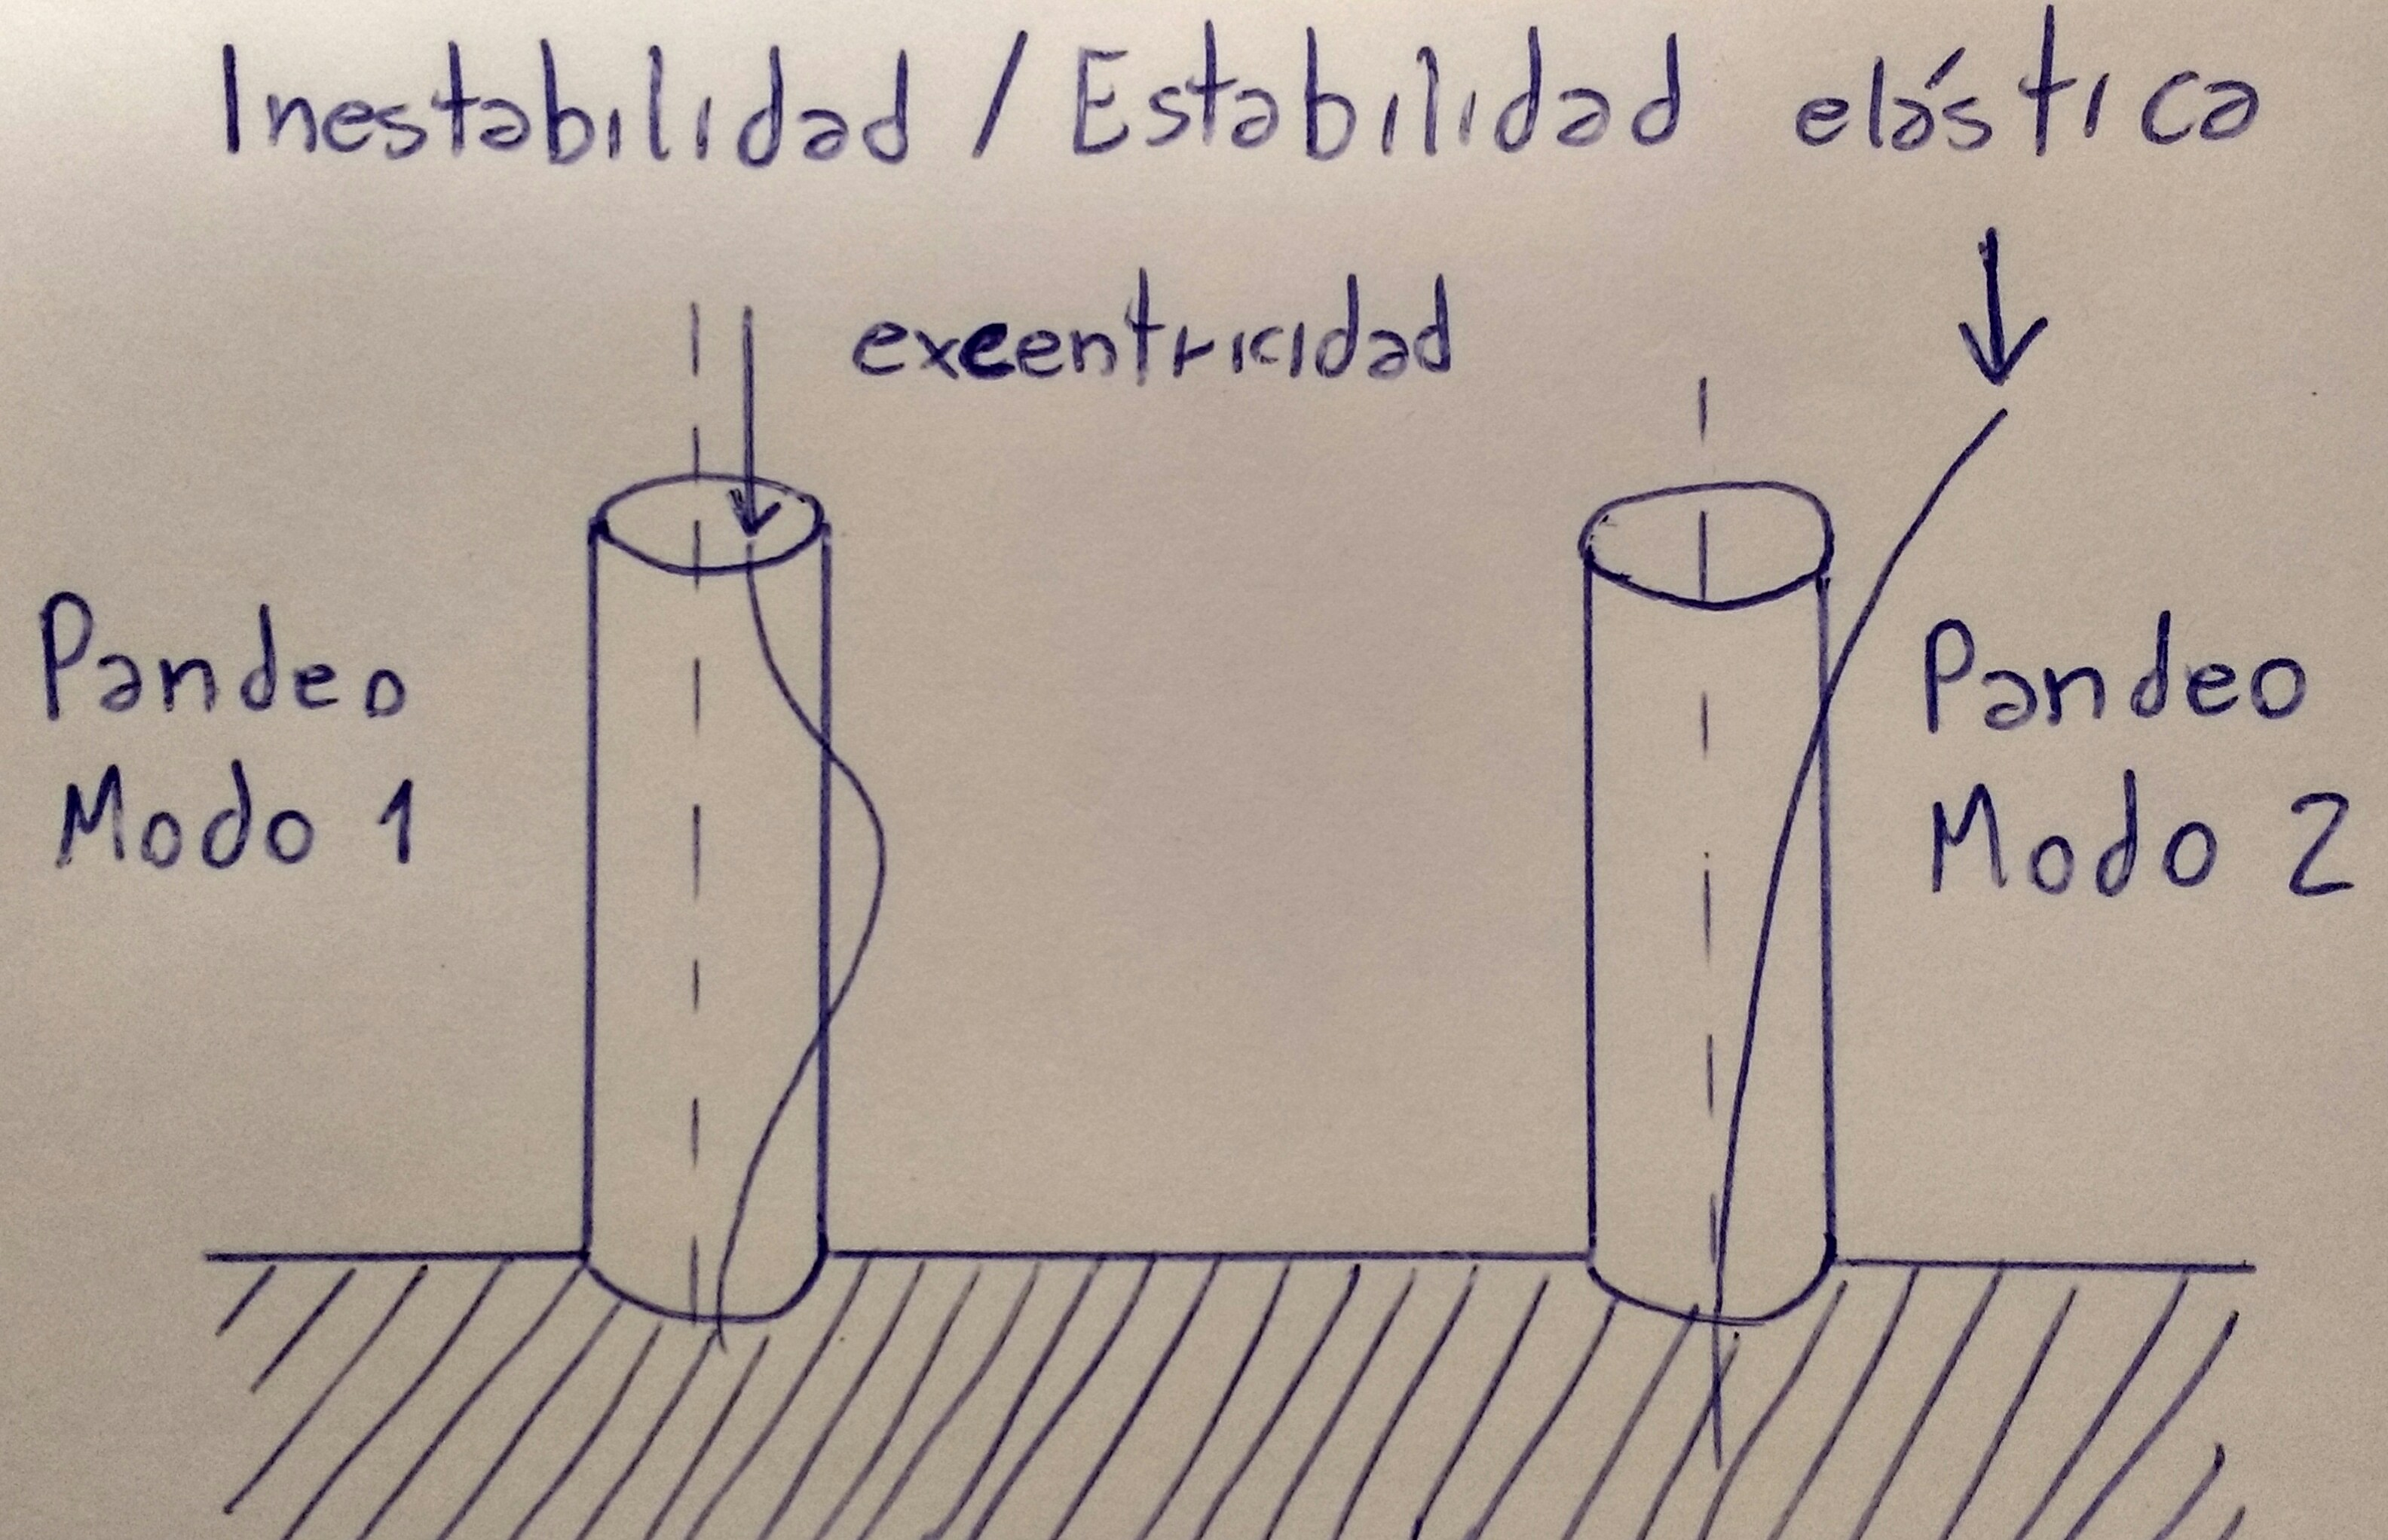
\includegraphics[width=0.6\linewidth,keepaspectratio]{6.jpg}
\end{center}

\section*{Ejercicio 10}

Considere un estado bidimensional de tensiones en una placa delgada en la cual $\sigma_{z}=\tau_{zx}=\tau_{zy}=0$. Las ecuaciones de equilibrio actuando en la placa con cargas distribuidas de cuerpo $X,Y$ (constantes) son:

\[
\frac{\partial\sigma_{x}}{\partial x}+\frac{\partial\tau_{xy}}{\partial y}+X=0;\quad\frac{\partial\tau_{xy}}{\partial x}+\frac{\partial\sigma_{y}}{\partial y}+Y=0
\]

Mostrar que estas ecuaciones se satisfacen idénticamente si $\sigma_{x},\sigma_{y},\tau_{xy}$ se derivan de una función arbitraria $\Phi(x,y)$ en la forma:

\[
\sigma_{x}=\frac{\partial^{2}\Phi}{\partial y^{2}};\quad
\sigma_{y}=\frac{\partial^{2}\Phi}{\partial x^{2}};\quad
\tau_{xy}=-\frac{\partial^{2}\Phi}{\partial x\partial y}-Xy-Yx
\]

Luego, las ecuaciones de equilibrio pueden ser satisfechas por infinitas soluciones distintas. Veremos más adelante la forma de elegir de entre éstas soluciones, aquéllas 
que corresponden al problema particular en análisis.

Realice un programa en Matlab u Octave, en donde se grafiquen los campos de tensiones  para las funciones $\Phi(x,y)$ siguientes en una región rectangular. Asuma cargas de cuerpo nulas. Elija valores arbitrarios. Interprete los resultados.

\begin{enumerate}[a.]
\item $\Phi(x,y)=ax^{2}+bxy+cy^{2}$
	\begin{enumerate}[I.]
	\item $a\neq 0;\quad b=c=0$
	\item $b\neq 0;\quad a=c=0$
	\item $c\neq 0;\quad a=b=0$
	\end{enumerate}
\item $\Phi(x,y)=ax^{3}+bx^{2}y+cxy^{2}+dy^{3}$
	\begin{enumerate}[I.]
	\item $d\neq 0;\quad a=b=c=0$
	\item $a\neq 0;\quad b=c=d=0$
	\item $b\neq 0;\quad a=c=d=0$
	\end{enumerate}
\end{enumerate}

\dotfill

\[
\left(\begin{matrix}
\sigma_{x} & \tau_{xy} & 0\\
\tau_{yx} & \sigma_{y} & 0\\
0 & 0 & 0\\
\end{matrix}\right)
\]\\

\[
\frac{\partial\sigma_{x}}{\partial x}+\frac{\partial\tau_{xy}}{\partial y}+X=
\frac{\partial}{\partial x}\left(\frac{\partial^{2}\Phi}{\partial y^2}\right)+
\frac{\partial}{\partial y}\left(-\frac{\partial^2\Phi}{\partial x\partial y}-Xy-Yx\right)+X
\]
\[
=\frac{\partial^3\Phi}{\partial x\partial y^2}-\frac{\partial^3\Phi}{\partial x\partial y^2}-X+X=0
\]\\

\[
\frac{\partial\tau_{xy}}{\partial x}+\frac{\partial\sigma_{y}}{\partial y}+Y=
\frac{\partial}{\partial x}\left(-\frac{\partial^2\Phi}{\partial x\partial y}-Xy-Yx\right)+
\frac{\partial}{\partial y}\left(\frac{\partial^2\Phi}{\partial x^2}\right)+Y
\]
\[
-\frac{\partial^3\Phi}{\partial x^2\partial y}-Y+\frac{\partial^3\Phi}{\partial x^2\partial y}+Y=0
\]

Campos de tensiones a.:

\begin{center}
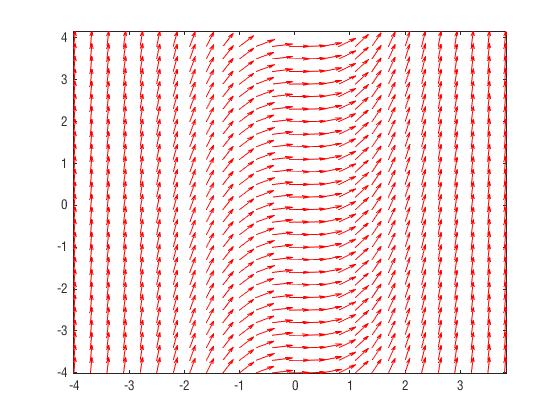
\includegraphics[width=0.6\linewidth,keepaspectratio]{g1.png}\\
I: $\Phi(x,y)=ax^2$

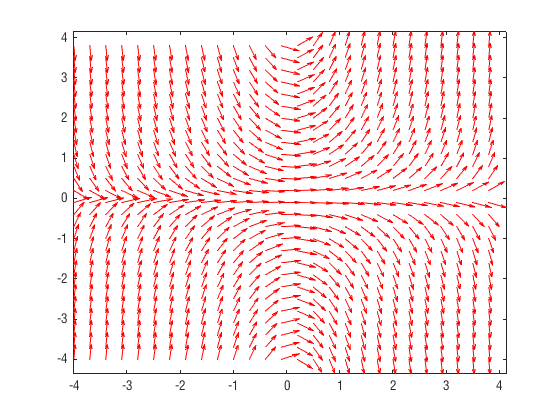
\includegraphics[width=0.6\linewidth,keepaspectratio]{g2.png}\\
II: $\Phi(x,y)=bxy$\\

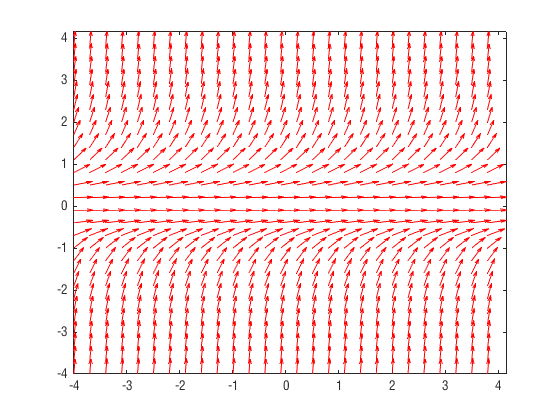
\includegraphics[width=0.6\linewidth,keepaspectratio]{g3.png}\\
III: $\Phi(x,y)=cy^2$
\end{center}

Campos de tensiones b.:

\begin{center}
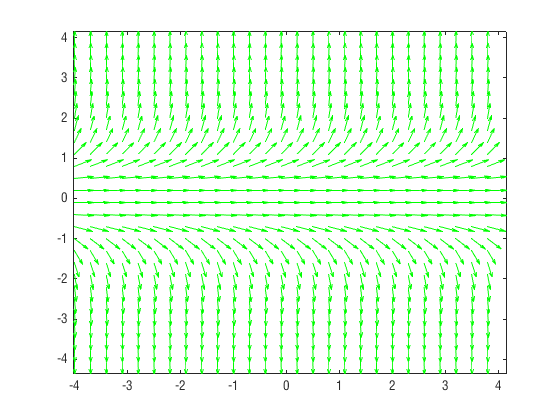
\includegraphics[width=0.6\linewidth,keepaspectratio]{g4.png}\\
I: $\Phi(x,y)=dy^3$

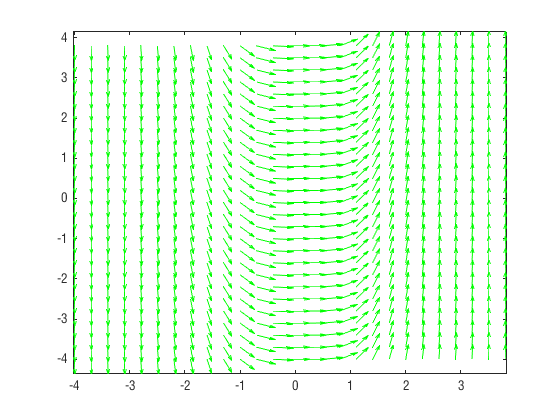
\includegraphics[width=0.6\linewidth,keepaspectratio]{g5.png}\\
II: $\Phi(x,y)=ax^3$\\

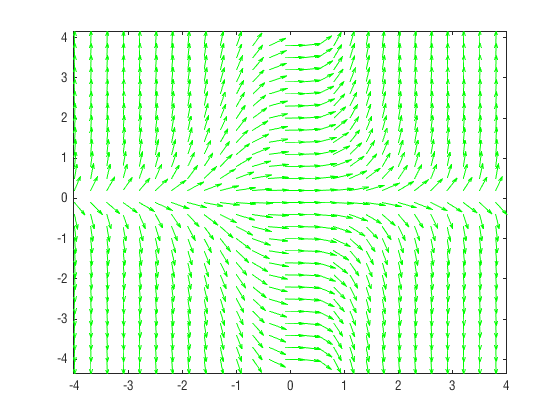
\includegraphics[width=0.6\linewidth,keepaspectratio]{g6.png}\\
III: $\Phi(x,y)=bx^{2}y$
\end{center}

\section*{Apéndice}

\textbf{Tensor de tensiones: }\textit{(Notación)}

\[
\sigma_{ij}=\tau_{ij}=
\left(\begin{matrix}
\sigma_{xx} & \sigma_{xy} & \sigma_{xz}\\
\sigma_{yx} & \sigma_{yy} & \sigma_{yz}\\
\sigma_{zx} & \sigma_{zy} & \sigma_{zz}\\
\end{matrix}\right)=
\left(\begin{matrix}
\sigma_{x} & \tau_{xy} & \tau_{xz}\\
\tau_{yx} & \sigma_{y} & \tau_{yz}\\
\tau_{zx} & \tau_{zy} & \sigma_{z}\\
\end{matrix}\right)=
\left(\begin{matrix}
\tau_{xx} & \tau_{xy} & \tau_{xz}\\
\tau_{yx} & \tau_{yy} & \tau_{yz}\\
\tau_{zx} & \tau_{zy} & \tau_{zz}\\
\end{matrix}\right)
\]

Son todas maneras diferentes de denotar lo mismo.\\

\textbf{Vector de tensión:}

\[
\stackrel \nu T_{i}=\sigma_{ij}\nu_{j}
\]

\[
\stackrel \nu T=T^{(n)}+T^{(c)};\quad T^{(c)}=\stackrel \nu T-T^{(n)};\quad T^{(n)}=(\stackrel \nu T\cdot\nu)\nu
\]

\begin{quote}
\textit{$\sigma$: tensor de tensiones.}\\
\textit{$\nu$: vector unitario normal al plano.}\\
\textit{$T^{(n)}$: componente normal del vector de tensión.}\\
\textit{$T^{(c)}$: componente tangencial del vector de tensión.}
\end{quote}

\textbf{Ecuaciones de equilibrio:}

\[
\textit{div }\sigma+\mathbf{X}=(\nabla\bullet\sigma)+\mathbf{X}=\frac{\partial\tau_{ji}}{\partial x_{j}}+X_{i}=
\tau_{ji,j}+X_{i}=0
\]

\begin{thebibliography}{1}
\bibitem{MCF}
Y. C. Fung,
\emph{A First Course in Continuum Mechanics}, 
tercera edición,
PRENTICE HALL,
1994.
\end{thebibliography}

\end{document}